\subsection{Business Process Models}

% O que é BPM

O BPM (Business Process Models) é uma abordagem sistemática para a gestão de processos de negócios que envolve o mapeamento, análise e melhoria dos processos para aumentar a eficiência, qualidade e eficácia. O método busca identificar as etapas envolvidas em um processo, as pessoas e sistemas envolvidos, bem como os principais indicadores de desempenho para monitorar e melhorar os resultados.

% De volta ao BPM

BPMs modelam uma série de etapas sequenciais que precisam ser realizadas para se completar uma tarefa ou processo específico, conhecidos como fluxo de trabalho. Eles são utilizados para definir como processos serão realizados, definindo objetivos dentro de uma organização~\cite{Alves2014UnderstandingOrganizations}. Eles podem ser utilizados para abstrair fluxos de trabalho existentes e criar novos fluxos com maior facilidade, podendo ser construídos seguindo uma das várias notação de BPMs, como a BPMN (Business Process Model and Notation)~\cite{Dijkman2008SemanticsBPMN}.

% BPMs (Business Process Models) são modelos de fluxos de trabalho utilizados para definir como processos serão realizados, definindo objetivos dentro de uma organização~\cite{Alves2014}. Eles podem ser utilizados para abstrair fluxos de trabalho existentes e criar novos fluxos com maior facilidade, podendo ser construídos seguindo a notação de BPMs, a BPMN (Business Process Model and Notation)~\cite{Dijkman2008}.

% Para que podem ser utilizados

BPMs são utilizados em uma ampla variedade de organizações, independente do setor ou do tipo de atividades. Sua aplicação ajuda as organizações a gerenciar e melhorar os seus processos de negócio, documentando como ele é feito e que passos devem ser seguidos para reprodução do mesmo~\cite{DaSilva2014BusinessNot}. Assim, os trabalhos podem ser melhor divididos entre os integrantes de uma equipe e pode-se encontrar falhas ou oportunidades de melhoria dentro de um processo.

% Onde são utilizados

% Exemplos de utilização

No setor de saúde, temos a utilização de BPM pelas instituições para gerenciar processos clínicos como atendimento ao paciente, gestão de agendamento, faturamento e gestão de registros médicos. Além disso, pedidos de exame e cadastro de amostras podem ser modelados para maior facilidade de compartilhamento de informações entre funcionários~\cite{Ruiz2012BusinessHealthcare.}.

% Introdução ao próximo capítulo LIMS e BPMS

BPMs são geralmente ilustrados com diagramas de fluxo, demonstrando um Fluxo de trabalho (workflow) com uma sequência de atividades e decisões tomadas no projeto~\cite{Entringer2021ComparativeStudy}, como pode ser visto no exemplo de método ágil modelado em BPM na figura~\ref{fig:bpm}.

A implementação de BPM dentro de uma organização ajuda a identificar pontos de melhoria no processo já instaurado, podendo aumentar a colaboração entre departamentos e garantir que o fluxo de trabalho seja feito de maneira eficiente e, principalmente, consistentemente~\cite{DaSilva2014BusinessNot}.
Além disso, os BPMs podem ajudar a monitoria e automatizar certos processos dentro de uma empresa, já que todos estarão bem documentados.

\begin{figure}
    \centering
    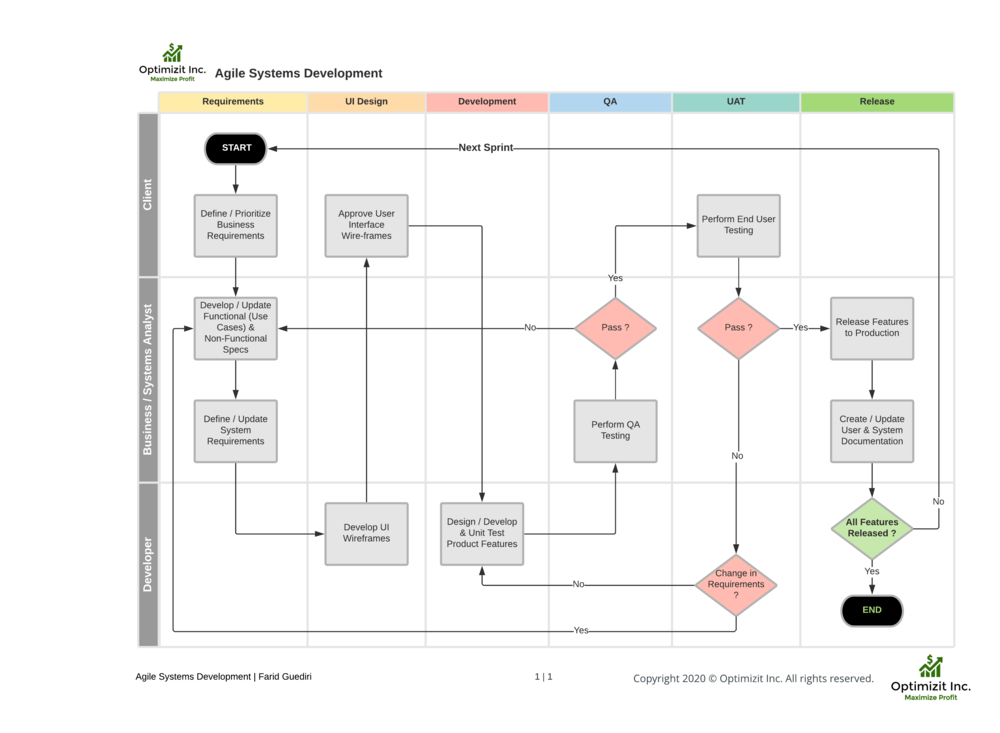
\includegraphics[width=1\textwidth]{imgs/BPM/sprint as bpm.png}
    \caption{Exemplos de um método ágil modelado como um BPM}
    \label{fig:bpm}
\end{figure}

% Comparação da utilidade dos sistemas e do BPM

BPMs podem ser utilizados com LIMS, para organizar o fluxo de trabalho dentro de um laboratório. Com isto, obtém-se uma maior automação de processos e um aumento da eficiência de cada etapa dentro de um determinado escopo~\cite{Key2011LIMS:Systems}.

Eles podem ser utilizados em conjunto pois tanto os sistemas de controle de acesso, coleta e análise de dados quanto o BPM têm como objetivo a automação e gerenciamento de processos complexos em uma organização. Ambos buscam melhorar a eficiência operacional, reduzir erros e aumentar a qualidade dos resultados.

É importante que o sistema esteja integrado com todos os passos do BPM modelado, especialmente em laboratórios e indústrias farmacêuticas, químicas e de biotecnologia, ajudando a melhorar a eficiência operacional, aumentando a precisão dos resultados e reduzindo erros com a automatização de tarefas repetitivas e da validação dos dados a serem colocados no sistema.

% É muito importante que um LIMS esteja integrado com partes do processo que são utilizadas para armazenar dados, como coleta e processamento de amostras em um ambiente laboratorial, pesquisa de dados dentro do programa para dados médicos, entre muitos outros, para que a sua implementação seja justificada e que o aumento de eficiência seja bem mensurado.

Para isso, utiliza-se LIMS que integram BPMs na construção de seus fluxos de trabalhos para que possam ser implementados em ambientes laboratoriais, seguindo todos os padrões necessários para sua implementação correta, garantindo a compatibilidade e a interoperabilidade entre diferentes sistemas utilizados, podendo ser utilizado por todos os funcionários da organização.

% Para isso, os LIMS devem ser personalizáveis para que possam ser integrados com outros sistemas que podem ser utilizados dentro da organização para garantir a compatibilidade e a interoperabilidade entre diferentes sistemas utilizados.